
\chapter{Coordinate transformations}
\label{ch:coordtrans}

% learning objective
\begin{lo3}[Coordinate transforms]
Determine components of a vector in a new coordinate system given the transformation matrix
\end{lo3}

\section{Rotation of coordinate axes}
\index{Coordinate transformation}

\begin{figure}[h]
\begin{center}
\framebox{
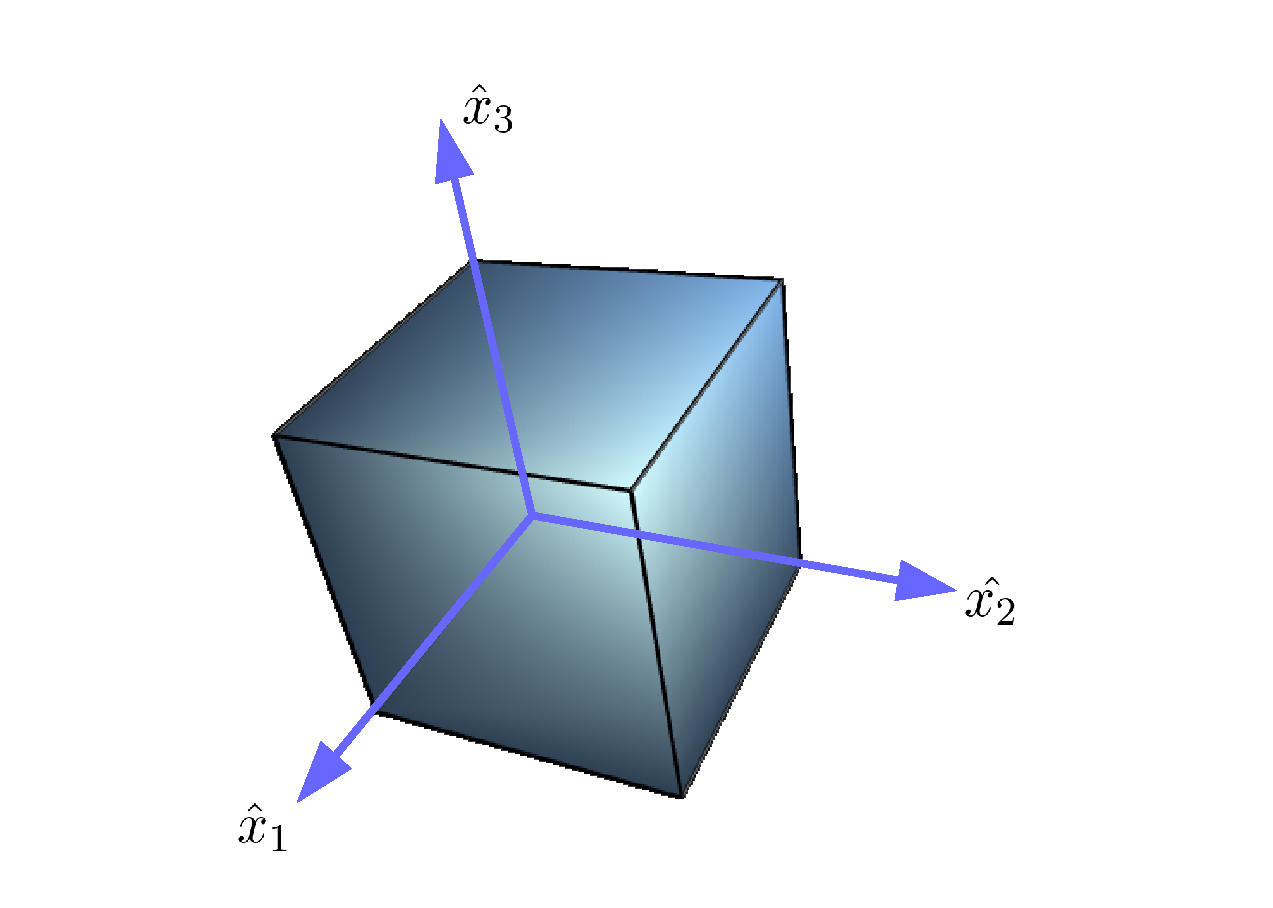
\includegraphics[scale=0.4]{images/c04-Orthogonality.eps}
 }
\end{center}
\caption{Orthogonal axes}
\label{orthogonalaxes1}
\end{figure}


Right-handed system: 
$$ \hat{x}_1 \cdot \left( \hat{x}_2 \times \hat{x}_3 \right) = 1 $$

$$ \hat{x}_1 \cdot \hat{x}_1 = \hat{x}_2 \cdot \hat{x}_2 = \hat{x}_3 \cdot \hat{x}_3 = 1 $$
$$ \hat{x}_1 \cdot \hat{x}_2 = \hat{x}_1 \cdot \hat{x}_3 = \hat{x}_2 \cdot \hat{x}_3 = 0 $$


If a coordinate system is rotated, how are the unit vectors of the two systems related?

\begin{figure}[h]
\begin{center}
\framebox{
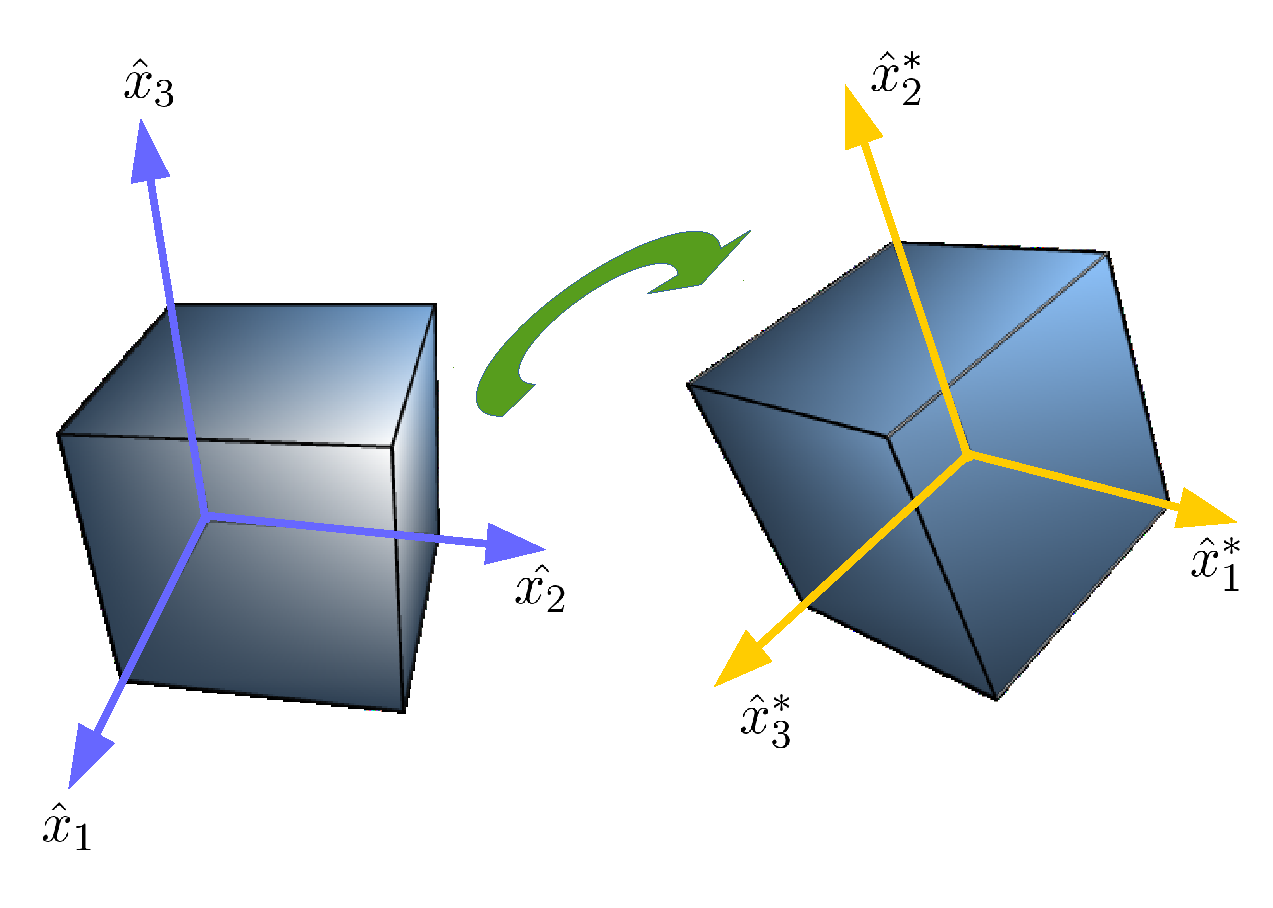
\includegraphics[scale=0.52]{images/c04-RotationIllustration.eps}
 }
\end{center}
\caption{Illustration of simple rotation of coordinate system}
\label{rotationofaxes}
\end{figure}



{\bf An example of coordinate transformation}

Consider rotating the coordinate system about $\hat{x}_3$ by an arbitrary angle $\theta$.

\begin{figure}[h]
\begin{center}
\framebox{
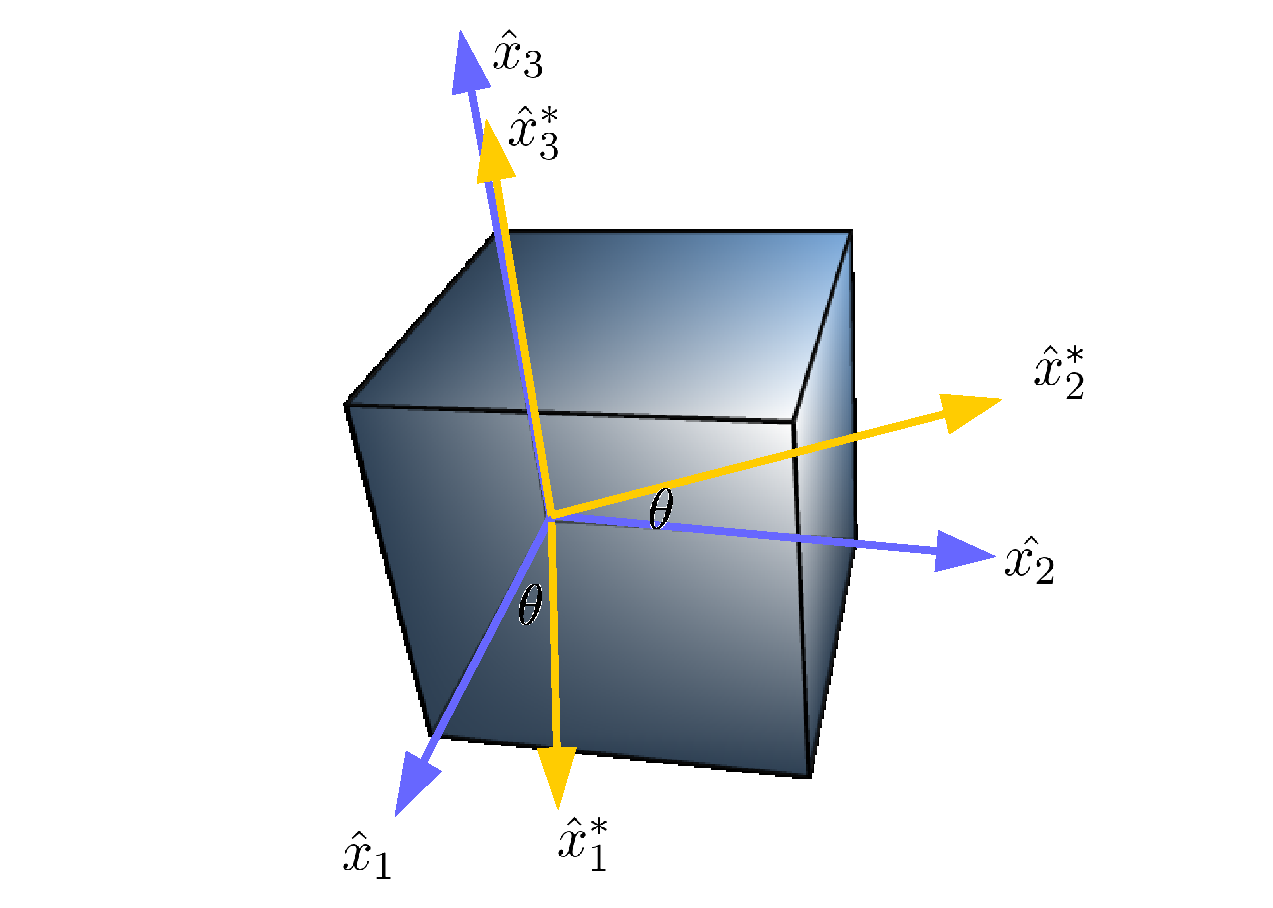
\includegraphics[scale=0.5]{images/c04-SimpleRotation.eps}
 }
\end{center}
\caption{Simple rotation about $\hat{x}_3$ axis}
\label{rotationofaxes2}
\end{figure}


{\bf New unit vectors in terms of old ones}

\begin{figure}[h]
\begin{center}
\framebox{
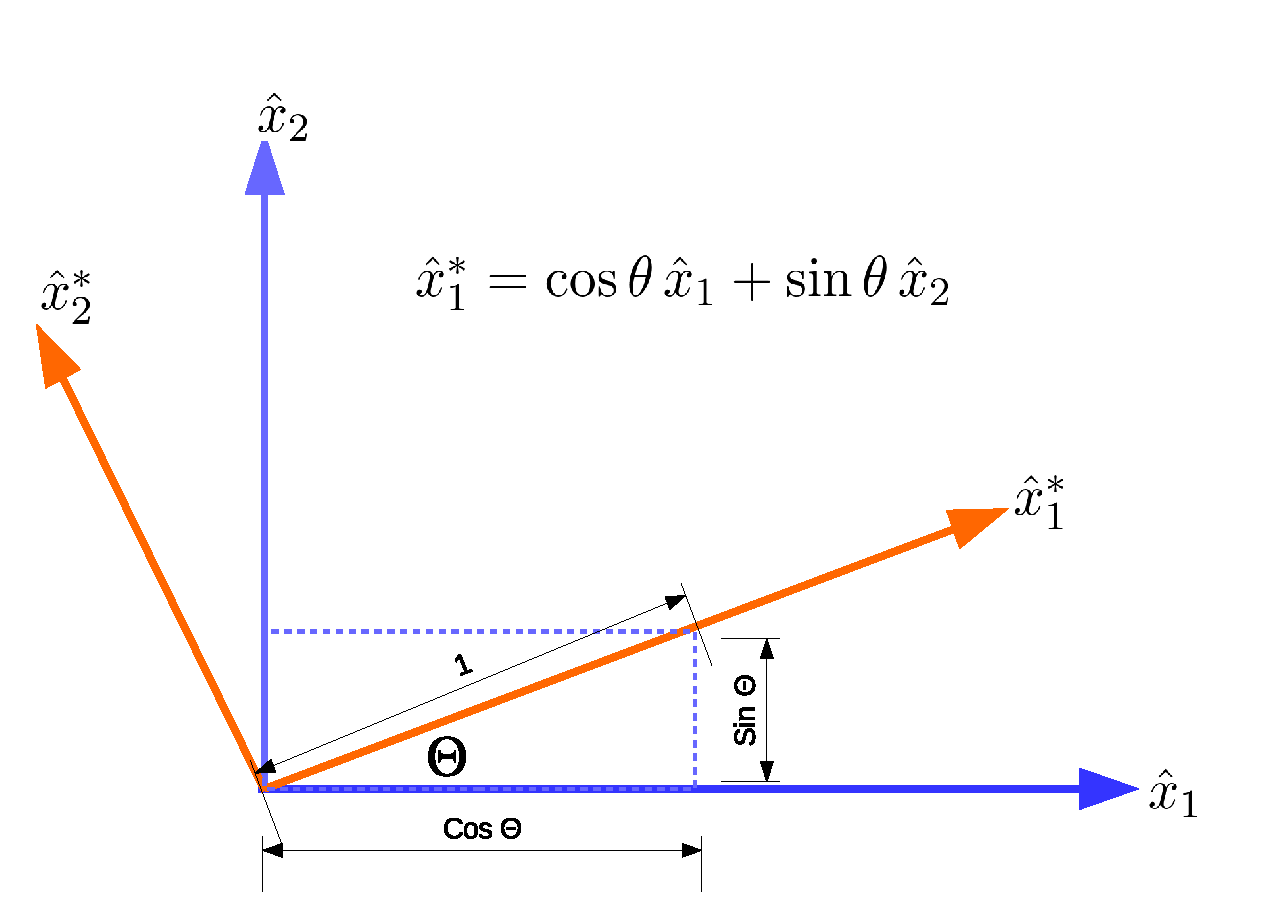
\includegraphics[scale=0.52]{images/c04-CoordinateRotations-1.eps}
 }
\end{center}
\caption{New unit vector $\hat{x}_1$ in terms of old ones after coordinate rotation}
\label{rotationofaxes3}
\end{figure}



\begin{figure}[h]
\begin{center}
\framebox{
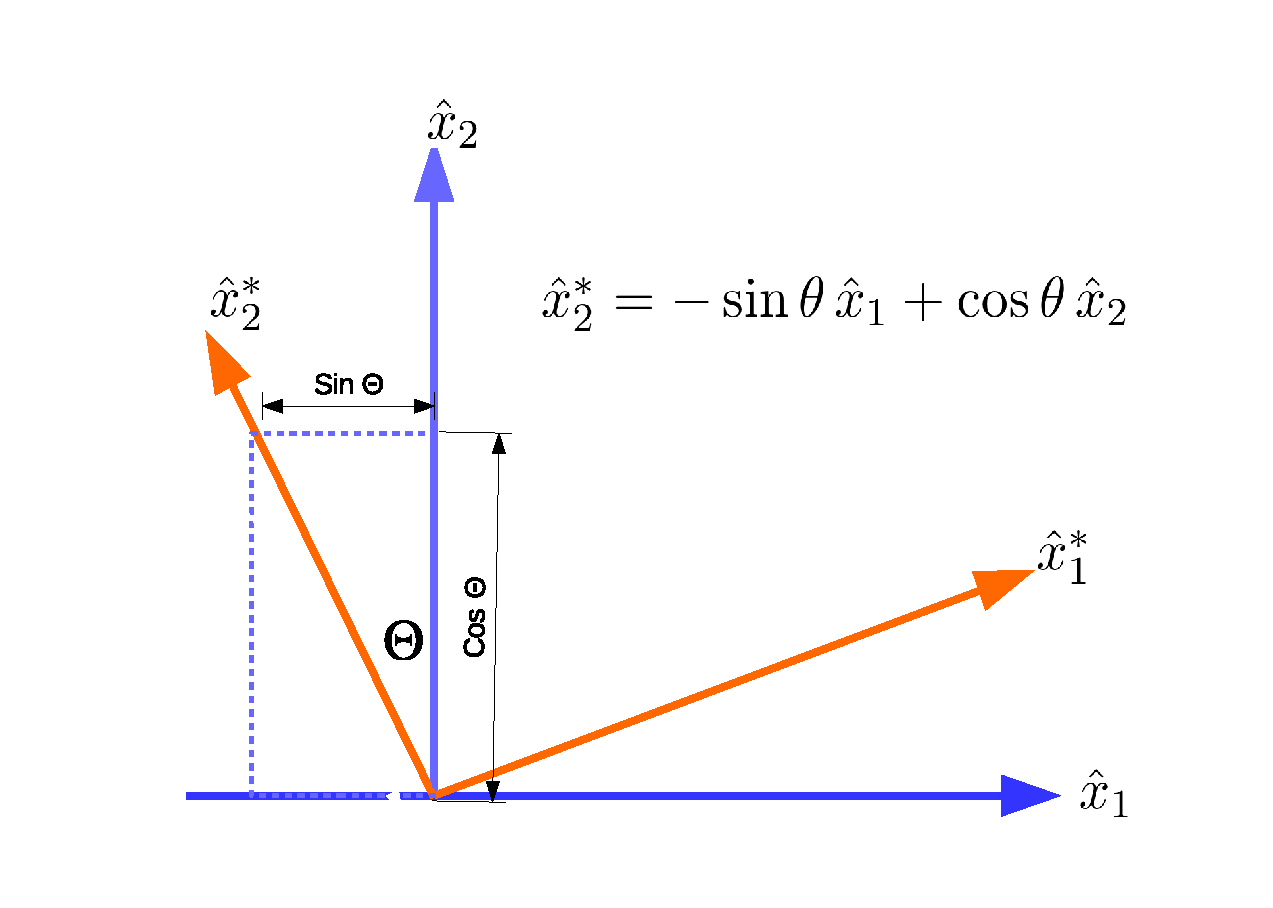
\includegraphics[scale=0.52]{images/c04-CoordinateRotations-2.eps}
 }
\end{center}
\caption{New unit vector $\hat{x}_2$ in terms of old ones after coordinate rotation}
\label{rotationofaxes4}
\end{figure}


$$ \hat{x}^*_1 = \cos\theta \, \hat{x}_1 + \sin\theta \, \hat{x}_2 + 0 \, \hat{x}_3 $$ 
$$ \hat{x}^*_2 = -\sin\theta \, \hat{x}_1 + \cos\theta \, \hat{x}_2 + 0 \, \hat{x}_3 $$ 
$$ \hat{x}^*_3 = 0 \, \hat{x}_1 + 0 \, \hat{x}_2 + \hat{x}_3 $$ 

or

\begin{equation*}
\left[ 
\begin{array}{l}
\hat{x}_1^*  \\
\hat{x}_2^* \\
\hat{x}_3^*  \\
\end{array}
\right] 
= \left[ 
\begin{array}{lll}
 \cos\theta  &  \sin\theta  & 0\\
 -\sin\theta &  \cos\theta  & 0 \\
  0 & 0 & 1\\
\end{array}
\right] 
\left[ 
\begin{array}{l}
\hat{x}_1 \\
\hat{x}_2 \\
\hat{x}_3 \\
\end{array}
\right]
\end{equation*}

\begin{equation*}
\left[ 
\begin{array}{l}
\hat{x}_1^*  \\
\hat{x}_2^* \\
\hat{x}_3^*  \\
\end{array}
\right] 
= \left[ 
\begin{array}{lll}
 T_{11}  &  T_{12}  & T_{13}\\
 T_{21}  &  T_{22}  & T_{23}\\
 T_{31}  &  T_{32}  & T_{33}\\
\end{array}
\right] 
\left[ 
\begin{array}{l}
\hat{x}_1 \\
\hat{x}_2 \\
\hat{x}_3 \\
\end{array}
\right]
\end{equation*}

Where
\begin{equation*}
T 
= \left[ 
\begin{array}{lll}
 \cos\theta  &  \sin\theta  & 0\\
 -\sin\theta &  \cos\theta  & 0 \\
  0 & 0 & 1\\
\end{array}
\right] 
\end{equation*}

Using subscript notation,

$$ \hat{x}^*_p = T_{pi} \hat{x}_i $$

{\bf Old unit vectors in terms of new ones}

\begin{figure}[h]
\begin{center}
\framebox{
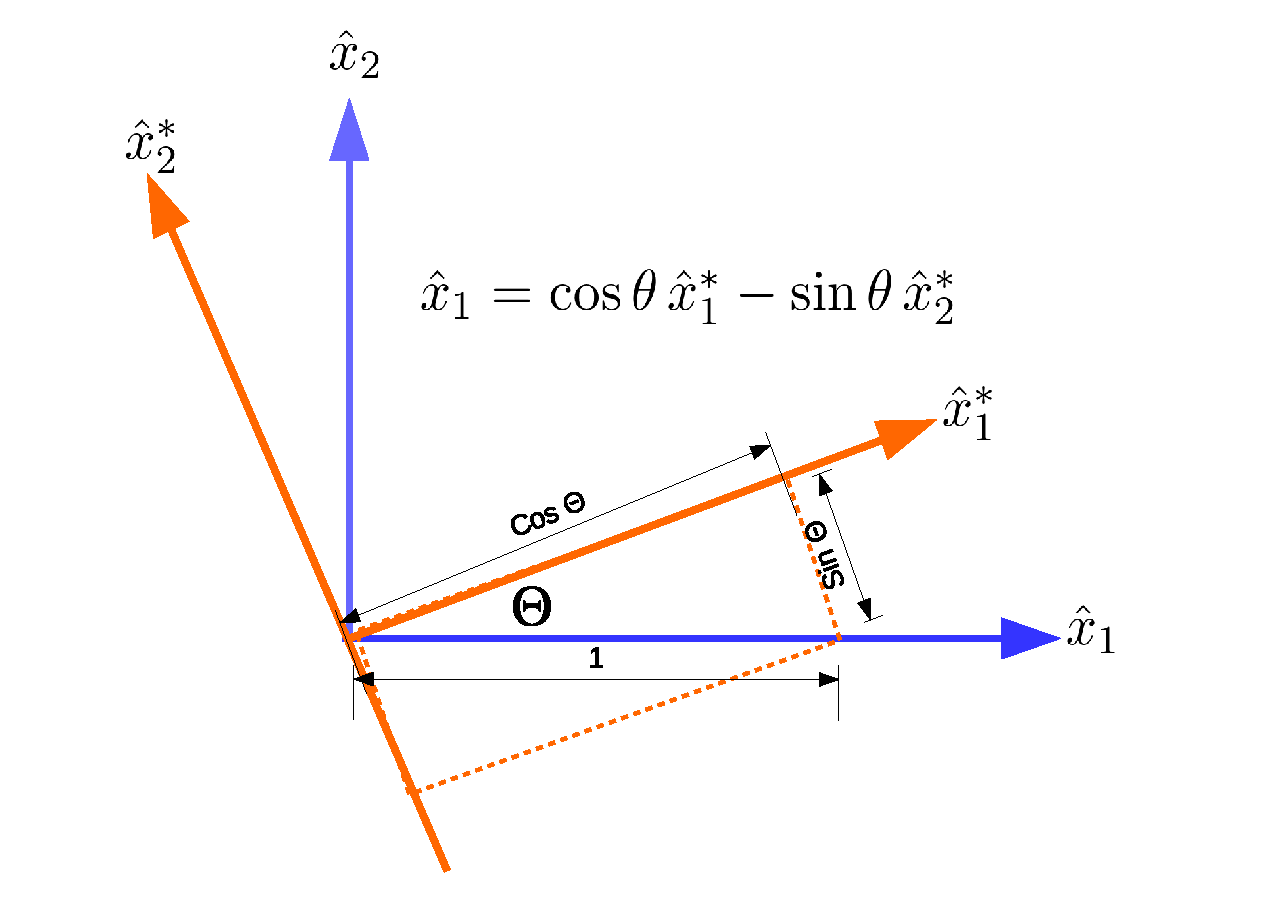
\includegraphics[scale=0.52]{images/c04-CoordinateRotations-3.eps}
 }
\end{center}
\caption{Old unit vector $\hat{x}_1$ in terms of new ones after coordinate rotation}
\label{rotationofaxes5}
\end{figure}



\begin{figure}[h]
\begin{center}
\framebox{
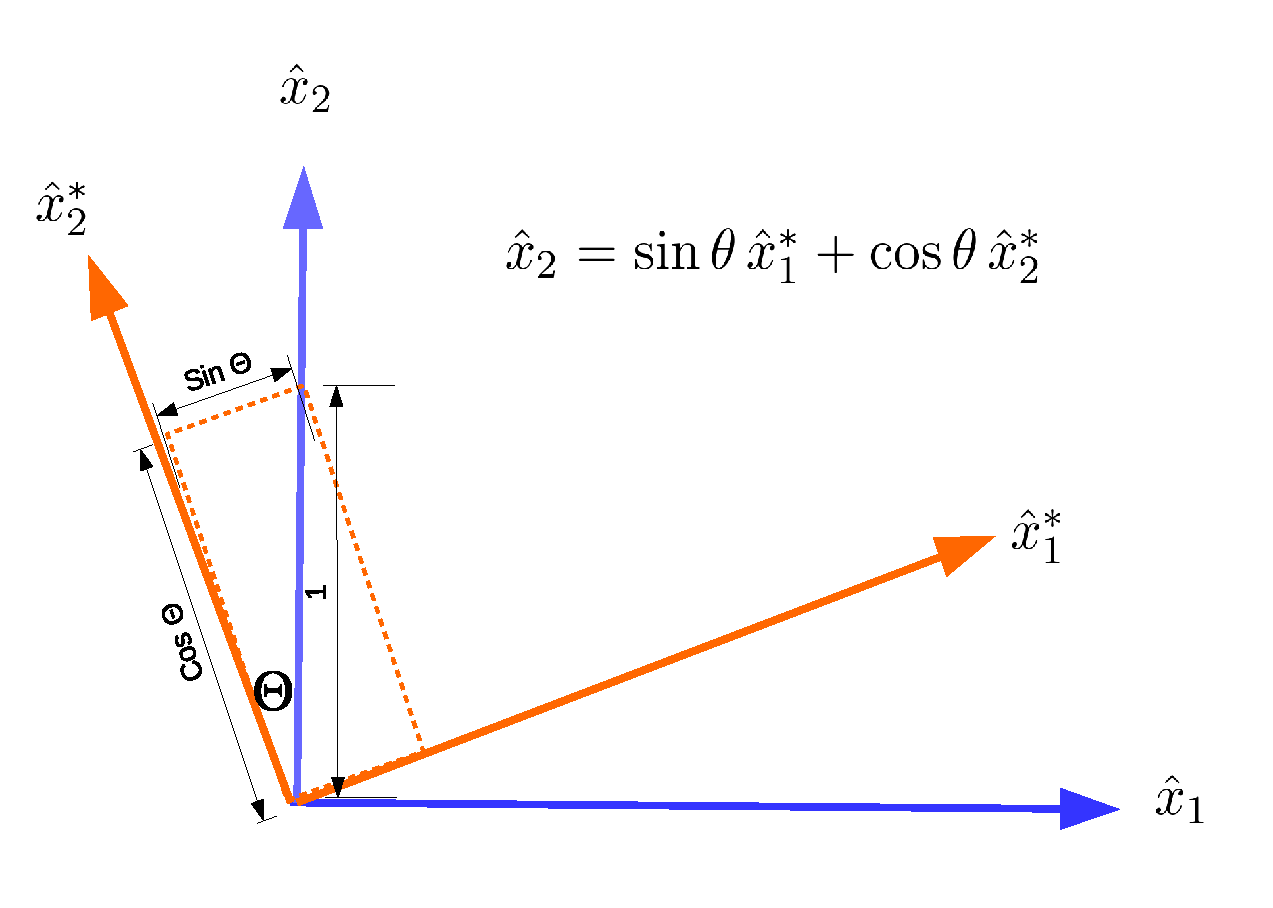
\includegraphics[scale=0.52]{images/c04-CoordinateRotations-4.eps}
 }
\end{center}
\caption{Old unit vector $\hat{x}_2$ in terms of new ones after coordinate rotation}
\label{rotationofaxes6}
\end{figure}



$$ \hat{x}_1 = \cos\theta \, \hat{x}^*_1 + -\sin\theta \, \hat{x}^*_2 + 0 \, \hat{x}^*_3 $$ 
$$ \hat{x}_2 = \sin\theta \, \hat{x}^*_1 + \cos\theta \, \hat{x}_2 + 0 \, \hat{x}_3 $$ 
$$ \hat{x}_3 = 0 \, \hat{x}^*_1 + 0 \, \hat{x}^*_2 + \hat{x}^*_3 $$ 

or

\begin{equation*}
\left[ 
\begin{array}{l}
\hat{x}_1  \\
\hat{x}_2 \\
\hat{x}_3  \\
\end{array}
\right] 
= \left[ 
\begin{array}{lll}
 \cos\theta  &  -\sin\theta  & 0\\
 \sin\theta &  \cos\theta  & 0 \\
  0 & 0 & 1\\
\end{array}
\right] 
\left[ 
\begin{array}{l}
\hat{x}^*_1 \\
\hat{x}^*_2 \\
\hat{x}^*_3 \\
\end{array}
\right]
\end{equation*}

Using subscript notation,

$$ \hat{x}_i = T_{pi} \hat{x}^*_p $$


{\bf Watch out the sequence of indices}

Transformation of old to new coordinate system:

$$ \hat{x}^*_p = T_{pi} \hat{x}_i $$
\begin{equation*}
\left[ 
\begin{array}{l}
\hat{x}_1^*  \\
\hat{x}_2^* \\
\hat{x}_3^*  \\
\end{array}
\right] 
= \left[ 
\begin{array}{lll}
T_{11} & T_{12} & T_{13} \\
T_{21} & T_{22} & T_{23} \\
T_{31} & T_{32} & T_{33} \\
\end{array}
\right] 
\left[ 
\begin{array}{l}
\hat{x}_1 \\
\hat{x}_2 \\
\hat{x}_3 \\
\end{array}
\right]
\end{equation*}

Transformation of new back to old coordinate system:

$$ \hat{x}_i = T_{pi} \hat{x}^*_p $$
\begin{equation*}
\left[ 
\begin{array}{l}
\hat{x}_1  \\
\hat{x}_2 \\
\hat{x}_3  \\
\end{array}
\right] 
= \left[ 
\begin{array}{lll}
T_{11} & T_{12} & T_{13} \\
T_{21} & T_{22} & T_{23} \\
T_{31} & T_{32} & T_{33} \\
\end{array}
\right] 
\left[ 
\begin{array}{l}
\hat{x}^*_1 \\
\hat{x}^*_2 \\
\hat{x}^*_3 \\
\end{array}
\right]
\end{equation*}


Watch out the sequence of indices !	

For old to new coordinate system, the convention is:

$$ \hat{x}^*_p = T_{pi} \hat{x}_i $$

Where, $p$ is the index for new- and $i$ is the index for old- coordinate systems.

{\bf Alternate definition of $T_{pi}$}

Consider the transformation from old to new coordinate system:
$$ \hat{x}^*_p = T_{pi} \hat{x}_i $$
Expand for $p=1$:
$$ \hat{x}^*_1 = T_{1i} \hat{x}_i = T_{11} \hat{x}_1 + T_{12} \hat{x}_2 + T_{13} \hat{x}_3 $$


This means one can also write the elements of $T_{pi}$ as

$$ T_{11} ={\partial \hat{x}^*_1 \over \partial \hat{x}_1 } $$
$$ T_{12} ={\partial \hat{x}^*_1 \over \partial \hat{x}_2 } $$
$$ T_{13} ={\partial \hat{x}^*_1 \over \partial \hat{x}_3 } $$

$$ T_{pi} = {\partial \hat{x}^*_p \over \partial \hat{x}_i} $$

% -----------------------------------------------------------------------


Consider the transformation from new to old coordinate system:
$$ \hat{x}_i = T_{pi} \hat{x}^*_p $$
Expand for $i=1$:
$$ \hat{x}_1 = T_{p1} \hat{x}^*_p = T_{11} \hat{x}^*_1 + T_{21} \hat{x}^*_2 + T_{31} \hat{x}^*_3 $$

Write the elements of $T_{pi}$ as
$$ T_{11} ={\partial \hat{x}_1 \over \partial \hat{x}^*_1 } $$
$$ T_{21} ={\partial \hat{x}_1 \over \partial \hat{x}^*_2 } $$
$$ T_{31} ={\partial \hat{x}_1 \over \partial \hat{x}^*_3 } $$

$$ T_{pi} = {\partial \hat{x}_i \over \partial \hat{x}^*_p} $$
$$ T_{pi} = {\partial \hat{x}^*_p \over \partial \hat{x}_i} = {\partial \hat{x}_i \over \partial \hat{x}^*_p}$$

{\bf Yet another definition of $T_{pi}$}

Consider the transformation from old to new coordinate system:
$$ \hat{x}^*_p = T_{pi} \hat{x}_i $$
Expand for $p=1$:
$$ \hat{x}^*_1 = T_{1i} \hat{x}_i = T_{11} \hat{x}_1 + T_{12} \hat{x}_2 + T_{13} \hat{x}_3 $$


This means one can also write the elements of $T_{pi}$ as

$$ \hat{x}^*_1 \cdot  \hat{x}_1 = T_{11} $$
$$ \hat{x}^*_1 \cdot \hat{x}_2 = T_{12} $$
$$ \hat{x}^*_1  \cdot \hat{x}_3 = T_{13} $$


$$ T_{pi} =  \hat{x}^*_p \cdot \hat{x}_i $$


% -----------------------------------------------------------------------

{\bf Properties of $T_{pi}$ using orthogonality}

$$ \hat{x}^*_1 \cdot \hat{x}^*_1 = 1 $$
$$ \hat{x}^*_1 = T_{1i} \hat{x}_i $$
$$ T_{1i} T_{1i} = 1 = \delta_{11} $$

$$ \hat{x}^*_1 \cdot \hat{x}^*_2 = 0 $$
$$ \hat{x}^*_1 = T_{1i} \hat{x}_i $$
$$ \hat{x}^*_2 = T_{2i} \hat{x}_i $$
$$ T_{1i} T_{2i} = 0 = \delta_{12} $$

$$ \hat{x}^*_1 \cdot \hat{x}^*_3 = 0 $$
$$ \hat{x}^*_1 = T_{1i} \hat{x}_i $$
$$ \hat{x}^*_3 = T_{3i} \hat{x}_i $$
$$ T_{1i} T_{3i} = 0 = \delta_{13} $$

Generalizing,

$$ T_{mi} T_{ni} = \delta_{mn} $$

Similarly, using the orthogonality of the old coordinate system, we can get

$$ T_{im} T_{in} = \delta_{mn} $$


% -----------------------------------------------------------------------

{\bf Properties of transformation matrix}

\begin{itemize}
\item $T_{pi}$ is determined by the rotation of the coordinate system
\item Determinant of $T_{pi}$ is 1
\item Inverse of $T_{pi}$ is its transpose, namely $T_{ip}$
\item Orthogonality leads to $ T_{mi} T_{ni} = \delta_{mn} $ and $ T_{im} T_{in} = \delta_{mn} $
\end{itemize}


% -----------------------------------------------------------------------

{\bf Components of a vector across coordinate rotation}

\begin{figure}[h]
\begin{center}
\framebox{
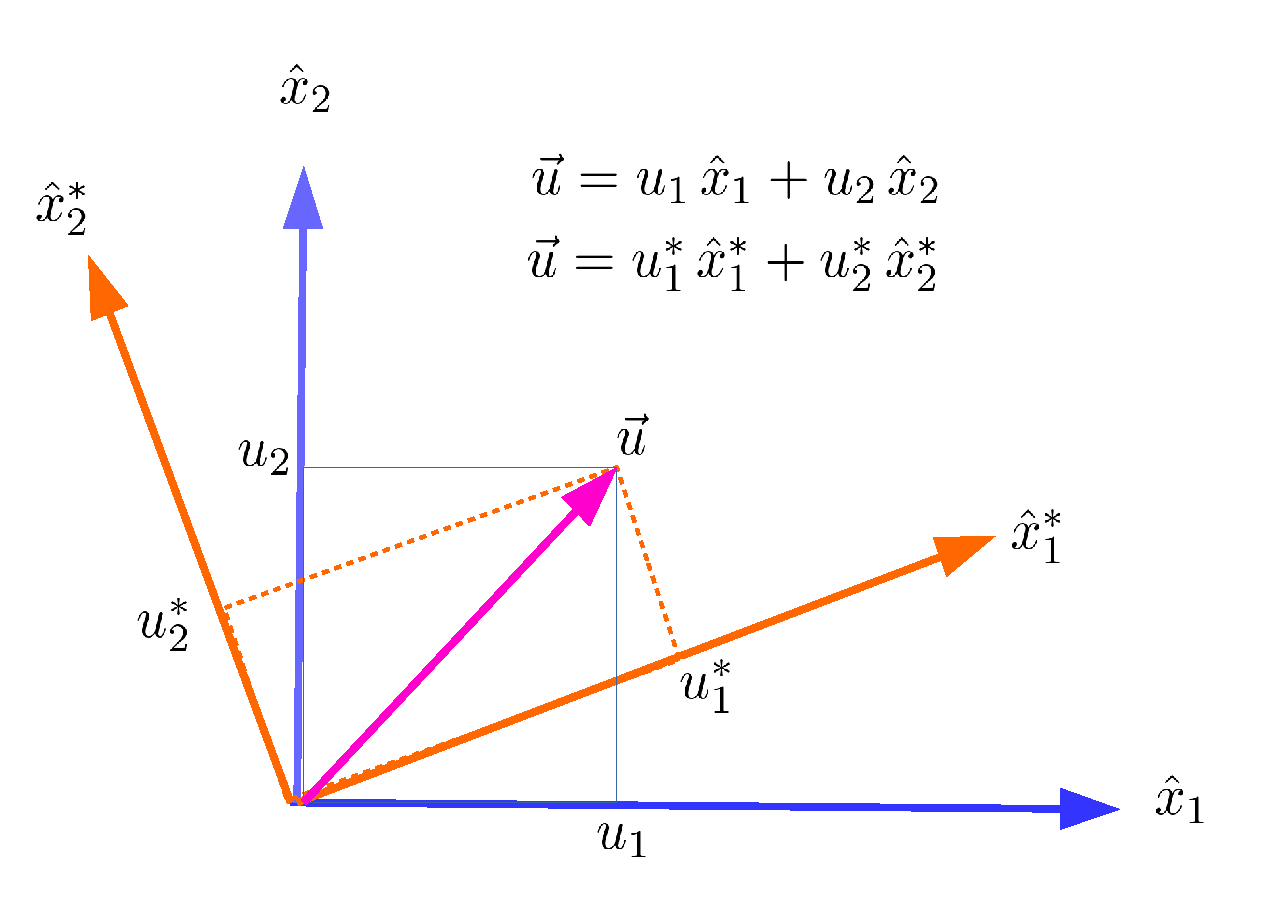
\includegraphics[scale=0.52]{images/c04-CoordinateRotations-5.eps}
 }
\end{center}
\caption{Components of a vector across coordinate rotation}
\label{rotationofaxes7}
\end{figure}


% -----------------------------------------------------------------------

{\bf Components of a vector across coordinate rotation}

$$ \vec{u} = u_1 x_1 + u_2 x_2 + u_3 x_3 $$
$$ = u_1 \left( \cos\theta \, \hat{x}^*_1 + \sin\theta \, \hat{x}^*_2 + 0 \, \hat{x}^*_3 \right) + $$
$$ + u_2 \left( -\sin\theta \, \hat{x}^*_1 + \cos\theta \, \hat{x}^*_2 + 0 \, \hat{x}^*_3 \right) +$$
$$ + u_3 \left( 0 \, \hat{x}^*_1 + 0 \, \hat{x}^*_2 + \hat{x}^*_3 \right) $$

$$ = \left( u_1 \cos\theta + u_2 \sin\theta \right) \hat{x}^*_2 + \left( -u_1 \sin\theta + u_2 \cos\theta \right) \hat{x}^*_2 + u_3 \hat{x}^*_3 $$

$$ = u^*_1 x^*_1 + u^*_2 x^*_2 + u^*_3 x^*_3  $$


% -----------------------------------------------------------------------

{\bf Components of a vector across coordinate rotation}

\begin{equation*}
\left[ 
\begin{array}{l}
u^*_1  \\
u^*_2 \\
u^*_3  \\
\end{array}
\right] 
= \left[ 
\begin{array}{lll}
 \cos\theta  &  \sin\theta  & 0\\
 -\sin\theta &  \cos\theta  & 0 \\
  0 & 0 & 1\\
\end{array}
\right] 
\left[ 
\begin{array}{l}
u_1 \\
u_2 \\
u_3 \\
\end{array}
\right]
\end{equation*}

or

$$ u^*_p = T_{pi} u_i $$

This equation preserves the nature of $\vec{u}$ across coordinate transforms and is thus a way to {\bf define} a vector.


% -----------------------------------------------------------------------

{\bf Definition of a vector}

A bunch of three numbers $u_i$ that follow the following relation across a coordinate transformation are components of a vector $\vec{u}$

{\bf Definition}
$$ u^*_p = T_{pi} u_i $$

A vector field is a vector that is a function of a location. 

{\bf Examples}
Velocity field $u\left(x,y,z\right)$, Gradient of thermal field $\vec{\nabla}T\left(r,\theta,z\right)$, Gradient of composition $\vec{\nabla}C_A\left(x,y,z\right)$, Electric field $E\left(x,y,z,\right)$ etc.,


% -----------------------------------------------------------------------

{\bf Definition of a scalar}

Scalar is a quantity which is invariant (does not change) across a coordinate transformation.

{\bf Examples}
Temperature $T$, Energy $G$, density $\rho$ etc.,

A scalar field is a scalar that is a function of location. 

{\bf Examples}
Thermal field $T\left(x,y,z\right)$, Density field $\rho\left(r,\theta,z\right)$, Phase field $\phi\left(x,y,z,\right)$ etc.,

Value of a scalar field at a location should not change if the coordinates chosen to represent the location change.


% ----------------------------------------------------------------------------------------

Cartesian co-ordinate system $\hat{x}_i$ is used. Consider the following co-ordinate transformation where the xy plane is rotated about z-axis clockwise by an angle $\theta$. 
\vspace{1cm}

%\begin{figure}[h]
% \centering
% \includegraphics[width=5 in]{images/ctrans0.eps}
% % ctrans.eps: 46x0 pixel, 300dpi, 0.39x0.00 cm, bb=0 35 595 420
% \caption{Co-ordinate Transformation}
% \label{ctrans}
%\end{figure}


The new axes (starred) are given in terms of the old axes (unstarred) by the following relations:

\begin{equation}
\begin{array}{l}
\hat{x}_1^* =  \hat{x}_1 cos\theta + \hat{x}_2 sin\theta \\
\hat{x}_2^* =  -\hat{x}_1 sin\theta + \hat{x}_2 cos\theta \\
\hat{x}_3^* =  \hat{x}_3 \\
\end{array}
\end{equation}
or
\begin{equation}
\label{oldnew}
\begin{array}{l}
\hat{x}_1^* = T_{11}\hat{x}_1 + T_{12}\hat{x}_2 + T_{13}\hat{x}_3\\
\hat{x}_2^* = T_{21}\hat{x}_1 + T_{22}\hat{x}_2 + T_{23}\hat{x}_3\\
\hat{x}_3^* = T_{31}\hat{x}_1 + T_{32}\hat{x}_2 + T_{33}\hat{x}_3\\
\end{array}
\end{equation}

\begin{equation}
\left( 
\begin{array}{l}
\hat{x}_1^*  \\
\hat{x}_2^* \\
\hat{x}_3^*  \\
\end{array}
\right) 
= \left( 
\begin{array}{lll}
 cos\theta  &  sin\theta  & 0\\
 -sin\theta &  cos\theta  & 0 \\
  0 & 0 & 1\\
\end{array}
\right) 
\left( 
\begin{array}{l}
\hat{x}_1 \\
\hat{x}_2 \\
\hat{x}_3 \\
\end{array}
\right)
\end{equation}

or

\begin{equation}
\label{vecdeff}
\boxed{
\hat{x}_p^* = T_{pi}\hat{x}_i
}
\end{equation} 

The transformation matrix \index{Transformation matrix} $T_{pi}$ used in the above expression is by the convention that first index represents the row and the second index, the column. In one of the reference texts, viz., Aris' book ~\cite{aris}, equation (2.11.1) shows that this convention is reversed. As a result the indices appear swapped in the definitions. This use of different convention is clear also from equation (A.6.4) in the same book.

When we express $x_i^*$ in terms of $x_i$, the {\bf transformation matrix} can be written as: 

\begin{equation}
T_{pi} = \frac{\partial \hat{x}_p^*}{\partial \hat{x}_i} =
\left( 
\begin{array}{lll}
\frac{\partial \hat{x}_1^*}{\partial \hat{x}_1} &
\frac{\partial \hat{x}_1^*}{\partial \hat{x}_2} &
\frac{\partial \hat{x}_1^*}{\partial \hat{x}_3} \\
\\
\frac{\partial \hat{x}_2^*}{\partial \hat{x}_1} &
\frac{\partial \hat{x}_2^*}{\partial \hat{x}_2} &
\frac{\partial \hat{x}_2^*}{\partial \hat{x}_3} \\
\\
\frac{\partial \hat{x}_3^*}{\partial \hat{x}_1} &
\frac{\partial \hat{x}_3^*}{\partial \hat{x}_2} &
\frac{\partial \hat{x}_3^*}{\partial \hat{x}_3} \\
\end{array}
\right) 
\end{equation}

We have chosen cartesian co-ordinate systems which have the following properties of {\em orthogonality} \index{Orthogonality}:

\begin{equation}
\label{ortho}
\begin{array}{lll}
\hat{x}^*_1 \cdot \hat{x}^*_1 = 1 & \hat{x}^*_2 \cdot \hat{x}^*_3 = 0 & \hat{x}^*_3 \cdot \hat{x}^*_2 = 0  \\
\hat{x}^*_2 \cdot \hat{x}^*_2 = 1 & \hat{x}^*_3 \cdot \hat{x}^*_1 = 0 & \hat{x}^*_1 \cdot \hat{x}^*_3 = 0  \\
\hat{x}^*_3 \cdot \hat{x}^*_3 = 1 & \hat{x}^*_1 \cdot \hat{x}^*_2 = 0 & \hat{x}^*_3 \cdot \hat{x}^*_1 = 0 \\
\end{array} 
\end{equation} 


Expressing $\hat{x}^*$ in terms of $\hat{x}$ and using equations~\ref{oldnew} and \ref{ortho}, we get:

\begin{equation}
\begin{array}{l}
T_{11}T_{12} + T_{21}T_{22} + T_{31}T_{32} = 0 \\
T_{12}T_{13} + T_{22}T_{23} + T_{32}T_{33} = 0 \\
T_{13}T_{11} + T_{23}T_{21} + T_{33}T_{31} = 0 \\
T_{11}T_{11} + T_{12}T_{12} + T_{13}T_{13} = 1 \\
T_{21}T_{21} + T_{22}T_{22} + T_{23}T_{23} = 1 \\
T_{31}T_{31} + T_{32}T_{32} + T_{33}T_{33} = 1
\end{array} 
\end{equation} 

or 

\begin{equation}
\boxed{
T_{ij}T_{ik} = \delta_{jk} 
}
\end{equation} 

{\bf Rotating the co-ordinate system back...}

Similarly, we can express $\hat{x}$ in terms of $\hat{x}^*$. Inverse transformation relation is given using the transpose of the transformation matrix as follows. Transpose of a matrix is nothing but the same matrix with the indices swapped around.
$$ \hat{x}_i = D_{ip} \hat{x}_p^*$$

The co-ordinate transformation matrix $D$ for new to old system is related to the matrix for old to new the following manner.

$$ D_{ip} = T_{ip}^{-1}= T_{ip}^{T} = T_{pi} $$

$$ \hat{x}_i = D_{ip} \hat{x}_p^* = T_{pi} \hat{x}_p^*$$

\begin{equation}
\label{vecdefr}
\boxed{\hat{x}_i = T_{pi} \hat{x}_p^*}
\end{equation}

{\bf Note:} Compare equations \ref{vecdeff} and \ref{vecdefr} and notice which of the indices is being repeated in the RHS.

Exploiting the orthogonality of the old co-ordinate system:

\begin{equation}
\begin{array}{lll}
\hat{x}_1 \cdot \hat{x}_1 = 1 & \hat{x}_2 \cdot \hat{x}_3 = 0 & \hat{x}_3 \cdot \hat{x}_2 = 0 \\
\hat{x}_2 \cdot \hat{x}_2 = 1 & \hat{x}_3 \cdot \hat{x}_1 = 0 & \hat{x}_1 \cdot \hat{x}_3 = 0 \\
\hat{x}_3 \cdot \hat{x}_3 = 1 & \hat{x}_1 \cdot \hat{x}_2 = 0 & \hat{x}_2 \cdot \hat{x}_3 = 0 \\
\end{array} 
\end{equation} 


\begin{equation}
\boxed{
T_{ji}T_{ki} = \delta_{jk}
}
\end{equation} 


\section{Scaffold to determine transformation matrix}

\begin{mdframed}[style=tpscaffold1]
\begin{enumerate}

\item For a rotation of a coordinate system about $\hat{x}_3$ by 90 degrees, anti-clockwise, express the unit vectors of the new coordinate system in terms of those of the old coordinate system. Write down how the transformation matrix would look like.

\item For a rotation of a coordinate system about $\hat{x}_3$ by 90 degrees, clockwise, write down how the transformation matrix would look like.

\item Write the unit vectors of the new coordinate system $\hat{x}_i^*$ in terms of $T_{ij}$ and unit vectors of the old coordinate system $\hat{x}_i$. Use the orthogonality properties of the unit vectors in the new coordinate system and determine what values the expression $T_{ij}T_{ik}$ would take.

\item If the transformation matrix for coordinate system rotation from $\hat{x}_i$ (old) to $\hat{x}_p^*$ (new) is $T_{pi}$ then convince yourself that the transformation matrix for rotating the new coordinate system back to the old one is the transpose of $T_{pi}$.

\item Write the unit vectors of the old coordinate system $\hat{x}_i$ in terms of $T_{ij}$ and unit vectors of the new coordinate system $\hat{x}_p^*$. Use the orthogonality properties of the unit vectors in the new coordinate system and determine what values the expression such as $T_{ji}T_{ki}$ would take.

\item Based on the answers to the above questions, generalize a rule when two terms of type $T_{ij}$ were to come together in an expression that involves summation over any index.

\end{enumerate}
\end{mdframed}

\section{Rodrigues rotation formula}

% learning objective
\begin{lo3}[Coordinate transforms]
Determine components of a transformation matrix given the axis and angle of rotation of a rectangular coordinate system
\end{lo3}


The transformation matrix for rotation of a coordinate system about an arbitrary axis given by the unit vector $\hat{n}$ by an arbitrary angle $\theta$ is given by:

\begin{equation}
R_{ij} = \cos\theta \, \delta_{ij} + \left( 1 - \cos \theta \right) \, n_i \, n_j - \sin\theta \epsilon_{ijk} n_k
\end{equation}

\begin{equation}
\hat{n} = n_i \hat{i} + n_j \hat{j} + n_k \hat{k}
\end{equation}

\begin{equation}
n_i^2 + n_j^2 + n_k^2 = 1
\end{equation}

The transformation matrix when expanded looks like the following.

\begin{align*}
\end{align*}

\begin{equation}
R_{ij}
= \left[ 
\begin{array}{lll}
\cos\theta + n_1^2\left( 1 - \cos\theta\right) & n_1 n_2 \left(1 - \cos\theta\right)-n_3 \sin\theta & n_1 n_3\left(1 - \cos\theta\right) + n_2 \sin\theta \\
n_1 n_2 \left( 1 - \cos\theta \right) + n_3 \sin\theta  &  \cos\theta + n_2^2 \left(1 - \cos\theta\right) & n_2 n_3\left(1 - \cos\theta\right) - n_1 \sin\theta \\
n_1 n_3 \left( 1 - \cos\theta \right) - n_2 \sin\theta & n_2 n_3 \left(1 - \cos\theta\right) + n_1 \sin\theta & \cos\theta + n_3^2 \left(1 - \cos\theta\right)  \\
\end{array}
\right] 
\end{equation}

One can substitute the values of $n_i$ for the unit vector $\hat{n}$ about which a rotation is being made, along with the value for $\theta$ for the angle of rotation and obtain the components of the transformation matrix $R_{ij}$ readily.

% ----------------------------------------------------------------------------

\begin{question}
	Show that the following matrix is a possible transformation matrix for coordinate rotation about a fixed point. 
\begin{equation}
T_{ij}
= \left[ 
\begin{array}{lll}
	\sin\theta \cos\phi & \sin\theta \sin\phi & \cos\theta \\
	\cos\theta \cos\phi & \cos\theta \sin\phi & -\sin\theta \\
	-\sin\phi & \cos\phi & 0
\end{array}
\right] 
\end{equation}

\end{question}
\begin{solution}[print]
	Show that the determinant is unity and that the orthogonality relations apply.
\end{solution}

% ----------------------------------------------------------------------------

\begin{question}
	If $T_{ij}$ is a transformation matrix, show that the following relations apply.
	$$ T_{11} = T_{22} T_{33} - T_{23} T_{32} $$
	$$ T_{12} = T_{23} T_{31} - T_{21} T_{33} $$
	$$ T_{13} = T_{21} T_{32} - T_{22} T_{31} $$

\end{question}
\begin{solution}[print]
	Consider the terms in $T_{ij}$ as direction cosines and compare the terms using the expression for determinant $\text{Det}\left(T_{ij}\right)=1$
\end{solution}

% ----------------------------------------------------------------

\section{Summary}

\begin{enumerate}
\item Orthogonality relations can be used to simplify terms while determining isotropy of a tensor
\end{enumerate}

% ----------------------------------------------------------------
